Nach einer kurzen Einarbeitung in Simspark und der Verwendung der ersten Frameworks, wurde klar, dass weder ein klassisches Logging, noch Debugging ausreichende Möglichkeiten bieten um eine schnelle Entwicklung zu ermöglichen. Durch Logging kann zwar der interne Ablauf nachvollzogen werden, jedoch sind serialisierte, dreidimensionale Vektoren wenig anschaulich.
Ein Debugging mit Breakpoints stört die Synchronisierung mit den Serverzyklen und ist somit noch eingeschränkter nutzbar. Deshalb wurde nach anderen Möglichkeiten der Analyse gesucht.

\subsection{RoboViz}
\label{subsec:RoboViz}
Der zusätzliche Monitor: 'RoboViz' ist ein Werkzeug, das genau für diesen Zweck entwickelt wurde. Er dient als Ersatz für den Standardmonitor von Simspark und ermöglicht ein zeichnen von zusätzlichen Informationen, direkt in der 3D-Szene. So können über geometrische Primitive und Textausgaben bei der Steuerung der NAOs anfallende Daten ausgeben werden. Dies geschieht in einer visuell schnell erfassbaren Weise, sodass Vektorumrechnungen oder -vorstellungen vermieden werden.\\

Der RoboViz nimmt über ein UDP-Socket die Debuginformationen in einem eigen Bytearray-Format entgegen. Die Befehle variieren in ihrer Länge, so nimmt eine Linie mehr Bytes entgegen, als ein Punkt. Gemein ist jedoch allen Befehlen, das diese mit einem 'set name' und einem Nullbyte abgeschlossen werden. Zu beachten ist, dass alle eingehenden Anweisungen mit dem selben 'set name' zunächst gesammelt werden. Erst nach einem 'swap buffer' Befehl werden alle diese gezeichnet. Sie sind solange sichtbar, bis der nächste 'swap buffer' eingeht.\\
Die mitgelieferte Java-Bibliothek ersetzt die Bytecodierung durch Methodenaufrufe mit entsprechenden Parametern.

\begin{figure}[H]
	\centering
	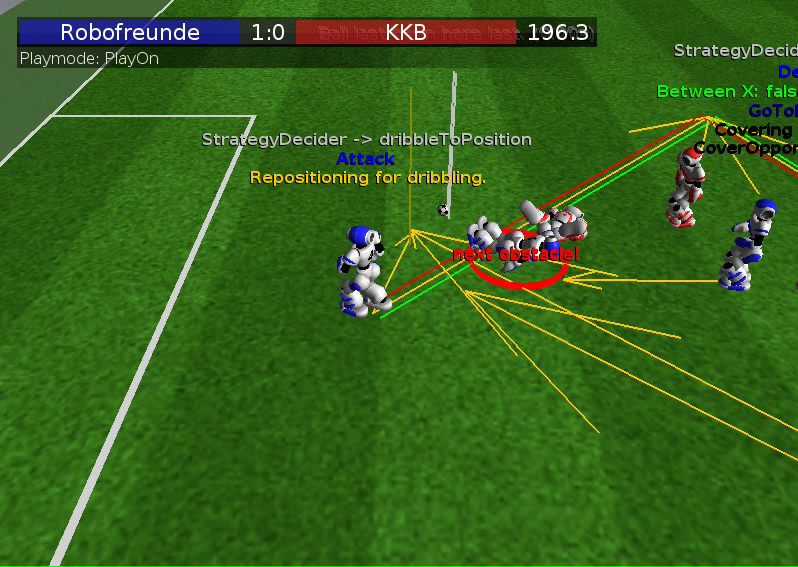
\includegraphics[width=\ScaleIfNeeded]{Grafiken/RoboViz/RoboVizzingToDaMax}
	\caption{Visualisierungen im Endspiel}
	\label{fig:roboviz-endgame}
\end{figure}


\subsection{Debugger}
\label{subsec:Debugger}
Um die Handhabung für die Entwicklung im Magma-Framework zu vereinfachen, wurde eine Debugger Schnittstelle geschaffen. Diese kapselt die Verwaltung der 'set name's sowie Farbcodes und konvertiert die Magma-typischen Vector3D-Elemente in die benötigten Parameter. Eine typische Ausgabe, wie sie beispielsweise beim Dribbeln erzeugt wird, wird so auf wenige Zeilen eingedampft:
\begin{lstlisting}[caption=RoboVizDebugger, captionpos=b, label=lst:Debug]
if (!getDebugger().isHidden()) {
   getDebugger().drawString("Repositioning for dribbling.", RoboVizColors.ORANGE);
   getDebugger().drawVector(getMyPosition(), dribbleStartPosition, RoboVizColors.ORANGE);
}
\end{lstlisting}

Zudem bietet der Debugger die Möglichkeit einen weiter abzuleiten, der dessen Socket mitverwendet und gleichzeitig einen eigenen 'set name' bekommt. Über Letzteren kann zur Laufzeit im RoboViz-Monitor die Ausgabe unterdrückt werden, ohne dass dies den ursprünglichen Debugger beeinflusst.

\begin{figure}[H]
	\centering
	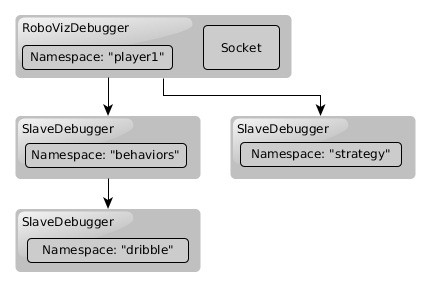
\includegraphics[width=240pt]{Grafiken/RoboViz/Debugger}
	\caption{Debugger - Beispiel-Hierarchie}
	\label{fig:debugger-hierarchy}
\end{figure}

Die entsprechen Klassen befinden sich in 'srcCommon/visualization'.

\subsection{Verteilung}
\label{subsec:Debugger Verteilung}
Um die Hierarchie der Debugger richtig aufzubauen, werden diese über ein 'Debuggable' Interface verteilt. Der Basis-Debugger wird in der Factory-Klasse der RoboFreunde erzeugt und dann an alle 'Behaviors' und 'DecisionMakers' verteilt, die das Interface implementieren. Daher ist es zum Debuggen notwendig das 'NaoRF'-Modell zu verwenden oder sich selbst um die Verteilung zu kümmern.\\
Wird kein Basis-Debugger erstellt, greifen die 'Debuggables' auf einen NullDebugger zurück, der standardmäßig versteckt ist und somit die anfallende Rechenlast minimiert.\\
Ein derartige, nachträgliches Verknüpfen der Komponenten außerhalb der Konstruktoren ermöglicht auch eine abwärts Kompatibilität zu anderen MetaModellen, die von RoboViz keine Ahnung haben.

\subsection{Debugger Graph}
\label{subsec:Debugger Graph}
Für eine einfachere Auswertung von Messwerten wurde eine Graph-Klasse erzeugt, die eine Reihe von Messwerten als Liniendiagramm darstellt. Beim Erstellen wird ein Ort für den Ursprung und ein Vektor, der sowohl Orientierung als auch Größe des Graphen festlegt übergeben. Ein übergebener Debugger dient als Ziel für alle Zeichenoperationen. Zum Darstellen der Daten können diese als Liste von Vector2D-Elementen übergeben werden. Die Skalierung der Achsen erfolgt automatisch und passt sich gegebenenfalls neuen Werten an. (Negative Werte sind ungetestet)\\
Der Graph sieht nicht nur toll aus und vereinfacht die Aufnahme von vielen Meßwerten für den Menschlichen Geist, er demonstriert auch eindrucksvoll wie Leistungsstark der RoboViz-Monitor bei der Darstellung auch sehr vieler Elemente ist.

\begin{figure}[H]
	\centering
	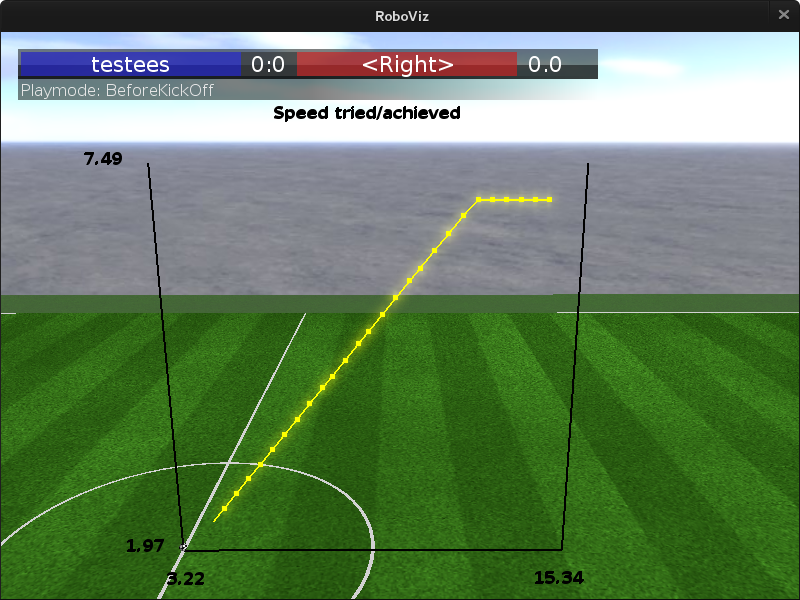
\includegraphics[width=\ScaleIfNeeded]{Grafiken/RoboViz/Graph}
	\caption{Debugger - Graph}
	\label{fig:debugger-graph}
\end{figure}